\section{Entropy of Uniformly Quantized Exponential Distribution}
\label{sec:003_entropy}

\emph{This post is about entropy of discrete stochastic variables that are derived by quantizing continuous stochastic variables. A good introduction to the concept of entropy in Information Theory is in \cite{Cover2012}.}

Let $x \in \{0\} \cup \mathbb{R}^+ $ be a continuous stochastic variable with $\text{Exponential}(\lambda)$ distribution and let $\hat{x} \in \{0\} \cup \hat{X}$ such that $\hat{X} \subset \mathbb{R}^+$ be its uniformly quantized version with step size $\Delta$. We would like to find the entropy of the discrete stochastic variable $\hat{x}$, denoted by $H_{\hat{x}}$, which provides us an estimate of the average number of bits required to encode $\hat{x}$.

For the continuous stochastic variable $x$, entropy is not generally defined. However, differential entropy, denoted by $h_x$, plays the same role as entropy for discrete stochastic variables. A well known approximation relating differential entropy of a variable and the entropy of its quantized version is given as follows.

\begin{align} H_{\hat{x}} \approx h_x - \log \Delta \end{align}

Unfortunately, this approximation is only valid for small values of $\Delta$ and breaks down as $\Delta$ increases. For example, for the common case of $\Delta = 1$, the approximation predicts the differential entropy and entropy of the quantized variable to be equal. This is generally not the case.

A common workaround is to use numerical simulations to calculate the $H_{\hat{x}}$. However, it would be satisfying to have an analytical expression notwithstanding its practical use. As we shall see below, the expression turns out to be quite cumbersome.

Let $\varphi(x)$ and $f(\hat{x})$ denote the probability density and mass functions of $x$ and $\hat{x}$ respectively. They are related as 
\begin{align}f(\hat{x}) = \int_{\hat{x} - [\hat{x} \neq 0]\frac{\Delta}{2}}^{\hat{x} + \frac{\Delta}{2}} \varphi(x) dx\end{align}. 
The indicator function $[\hat{x} \neq 0]$ is $0$ when $\hat{x} = 0$ and $1$ otherwise, and serves to set the lower bound correctly.

Now onto calculating the negative entropy $-H_{\hat{x}}$ which is given (by definition) as follows. The motivation behind using negative entropy instead of entropy is to avoid (many) negative signs on the right hand side expression.

\begin{align}-H_{\hat{x}} &= \sum_{\hat{x} \in \{0\} \cup \hat{X}} f(\hat{x}) \log f(\hat{x}) \\ &= \left(\int_{0}^{\frac{\Delta}{2}} \varphi(x) dx \right) \log \left[\int_{0}^{\frac{\Delta}{2}} \varphi(x) dx \right] \nonumber \\ &\quad + \sum_{\hat{x} \in \hat{X}} \left( \int_{\hat{x}-\frac{\Delta}{2}}^{\hat{x}+\frac{\Delta}{2}} \varphi(x) dx \right) \log \left[\int_{\hat{x}-\frac{\Delta}{2}}^{\hat{x}+\frac{\Delta}{2}} \varphi(x) dx \right]\end{align} 

Using the definition of the continuous distribution function for Exponential distribution, $\varphi(x) = \lambda e^{-\lambda x}$, the above equation is simplified as follows.

\begin{align} -H_{\hat{x}} &= \left(1-e^{-\lambda\frac{\Delta}{2}}\right) \log \left[ 1-e^{-\lambda\frac{\Delta}{2}} \right] \nonumber \\ &\quad + \left(e^{\lambda\frac{\Delta}{2}} - e^{-\lambda\frac{\Delta}{2}}\right) \log \left[e^{\lambda\frac{\Delta}{2}} - e^{-\lambda\frac{\Delta}{2}} \right] u_1(\lambda) \nonumber \\ &\quad +  \left(e^{\lambda\frac{\Delta}{2}} - e^{-\lambda\frac{\Delta}{2}}\right) u_2(\lambda) \label{eqn:hh} \end{align}
With the functions $u_{1,2}(\lambda)$ given by:
\begin{align} u_1(\lambda) &= \sum_{\hat{x} \in \hat{X}} e^{-\lambda\hat{x}} \\ u_2(\lambda) &= \sum_{\hat{x} \in \hat{X}} e^{-\lambda\hat{x}} \log e^{-\lambda\hat{x}} \end{align}

\subsection{Approximate Result}

The exact values of $u_{1,2}(\lambda)$, as we shall see below, are cumbersome. Therefore, we first obtain an approximate result by plugging in the the approximations for $u_{1,2}(\lambda)$ given below into equation (\ref{eqn:hh}).

\begin{align} u_1(\lambda) &= \frac{1}{\lambda} \sum_{\hat{x} \in \hat{X}} \lambda e^{-\lambda\hat{x}} \approx   \frac{1}{\lambda} \left[ \int_{0}^{\infty} \varphi(x) dx - \varphi(0) \right] = \frac{1}{\lambda} - 1\\ u_2(\lambda) &= \sum_{\hat{x} \in \hat{X}} e^{-\lambda\hat{x}} \log e^{-\lambda\hat{x}} \approx -\frac{h_x}{\lambda} - \log(\lambda)  - \log(\lambda) u_1(\lambda)\end{align}

The performance of the above approximation may be verified numerically. In the graph below, we hold quantization step size constant at $\Delta = 1$ and vary the parameter $\lambda$. We observe that the approximation is acceptable, i.e. bit difference < 1, for the range $0 < \lambda \leq 1.5$. For higher values of $\lambda$, the approximation fails.

\begin{figure}[H]
	\centering
	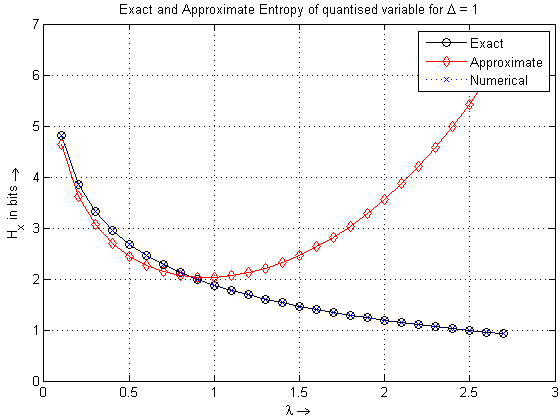
\includegraphics[width=0.95\textwidth,keepaspectratio]{003_001_approx1.png}
\end{figure}

\subsection{Exact Result}

The exact result, from the graph above, may be obtained by plugging in the exact values for $u_{1,2}(\lambda)$ into equation (\ref{eqn:hh}). The exact values may be computed starting from the following identities.

\begin{align} 1 &= \int_{0}^{\infty} \varphi(x) dx = \int_{0}^{\frac{\Delta}{2}} \varphi(x) dx + \sum_{\hat{x} \in \hat{X}} \int_{\hat{x} - \frac{\Delta}{2}}^{\hat{x} + \frac{\Delta}{2}} \varphi(x) dx \\ -h_x &= \int_{0}^{\infty} \varphi(x) \log \varphi(x) dx \nonumber \\ &= \int_{0}^{\frac{\Delta}{2}} \varphi(x) \log \varphi(x) dx + \sum_{\hat{x} \in \hat{X}} \int_{\hat{x} - \frac{\Delta}{2}}^{\hat{x} + \frac{\Delta}{2}} \varphi(x) \log \varphi(x) dx\end{align}

As the derivation is lengthy, we directly present the simplified result below.

\begin{align} u_1(\lambda) &= \frac{e^{-\lambda\frac{\Delta}{2}}}{e^{\lambda\frac{\Delta}{2}} - e^{-\lambda\frac{\Delta}{2}}} \\ u_2(\lambda) &= \frac{-h_x - c_1  - \frac{\Delta}{2}\lambda  \left[e^{\lambda\frac{\Delta}{2}} + e^{-\lambda\frac{\Delta}{2}}\right] u_1(\lambda)}{e^{\lambda\frac{\Delta}{2}} - e^{-\lambda\frac{\Delta}{2}}}\end{align}

Where $c_1 = log(\lambda) - 1 + \frac{\Delta}{2}\lambda e^{-\lambda\frac{\Delta}{2}}$. We see that even with a simple distribution function, the exact expressions quickly get out of hand and are unfortunately not short and elegant as one would have expected.

\subsection{Version History}
\begin{enumerate}
	\item \emph{First published: 3rd Oct. 2015 on aravindhk-math.blogspot.com}
	\item \emph{Modified: 16th Dec. 2023 -- Style updates for \LaTeX}
\end{enumerate}
